%!TEX encoding = UTF-8
\documentclass[a4paper]{jsarticle}
\usepackage[a4paper,margin=30truemm]{geometry}
\usepackage[dvipdfmx]{graphicx}
\usepackage{url}

\usepackage{layout}

\usepackage[dvipdfmx]{hyperref}
\usepackage{pxjahyper}

\hypersetup{%
colorlinks=true,
linkcolor=black,
citecolor=black,
urlcolor=black
}

\title{\vspace{-2cm}
  クマ財団 ポートフォリオ資料 \\
  Zwin : XR Windowing System
}
\author{
  木内 陽大
}

\begin{document}

\maketitle

\begin{figure}[htbp]
  \centering
  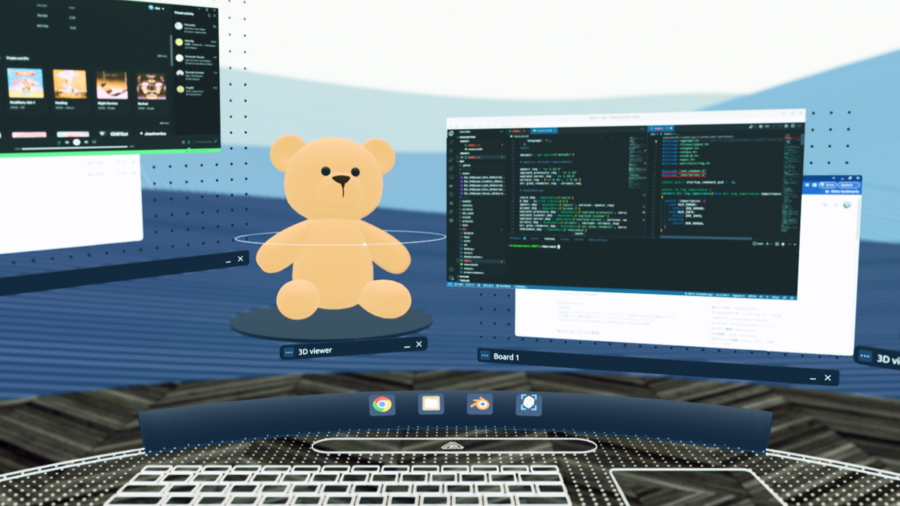
\includegraphics[width=\linewidth]{figure/hero2.png}
\end{figure}

\section{概要}

私のポートフォリオでは,自分が発足し,取り組んでいるプロジェクト
Zwin: XR Windowing Systemを紹介する.

\subsection{Windowing Systemとは}

通常コンピュータのGUIデスクトップ環境では,ブラウザやチャットツールなどのアプリケーションは
ウィンドウという形で起動される.
これによって複数のアプリケーションを立ち上げることができ,
それぞれのウィンドウが重なる形でデスクトップ環境が構成される.
ウィンドウが重なるように表現して合成しつつ,実際にディスプレイに映像を送っているのは
ディスプレイサーバというバックグラウンドアプリケーションであり,個々のアプリケーションは
このディスプレイサーバとやり取りをし,ウィンドウ内に描画したいコンテンツを伝えることで,
ディスプレイサーバにコンテンツを表示してもらっている(図\ref{fig:windowing-system}).
Windowing Systemはこの仕組み全体を表し,ディスプレイサーバとアプリケーションとの間の具体的な
やりとりのプロトコルなどを定めているものにはX\footnote{\url{https://www.x.org/wiki/}}や
Wayland\footnote{\url{https://wayland.freedesktop.org/}}などがある.

\begin{figure}[htbp]
  \centering
  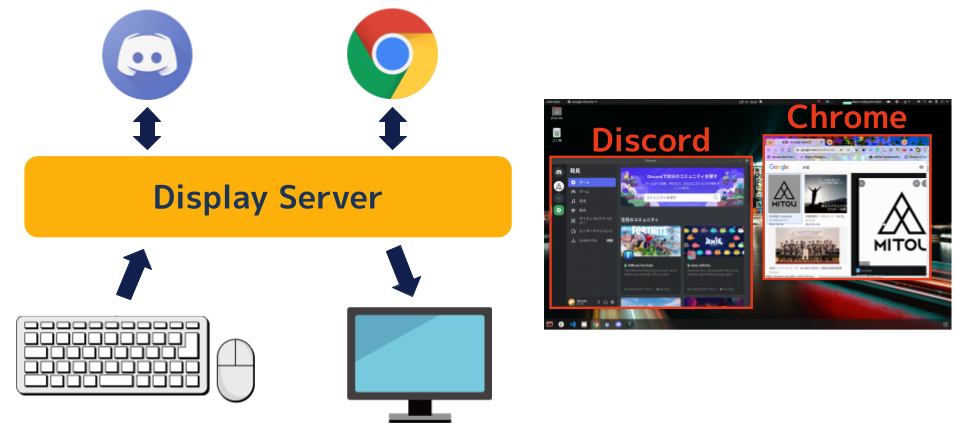
\includegraphics[width=\linewidth]{figure/windowing-system.png}
  \caption{
    Windowing Systemのしくみ.
    ディスプレイサーバはマウスやキーボードなどの入力を適切にアプリケーションに振り分け,
    アプリケーションからコンテンツの情報を受け取り,合成して,ディスプレイに表示する.
  }
  \label{fig:windowing-system}
\end{figure}

\subsection{Zwin}

ZwinではWindowing Systemの概念をXRに取り込むことで,XRで複数のアプリケーションを立ち上げる
ことを可能にした.
まずは35秒ほどの短い動画があるので実際に動いている様子をご覧いただきたい.

\url{https://youtube.com/shorts/aPeacvIrVMo?feature=share}

利用例として,図\ref{fig:zwin}ではVRの中で,Blender, Google Chromeといった
既存の2D アプリケーションを利用しつつ,Blenderで作成した世界をその場に表示したり,
アセットとなるオブジェクトをその場に表示して,大きさを確認したりできる様子を示している.
XRコンテンツを作る際に,コンテンツの作成と確認をXR内で完結できるため,HMDをいちいち着脱する
必要がなく,マルチディスプレイでの作業もできる.

またプロトタイプでは,図\ref{fig:zwin2}のようにGoogle Chromeと
3Dアプリケーションとの間でのドラッグ \& ドロップも実現しており,
天体のテクスチャをブラウザからドラッグ \& ドロップして張り替えることが可能である.

\begin{figure}[htbp]
  \centering
  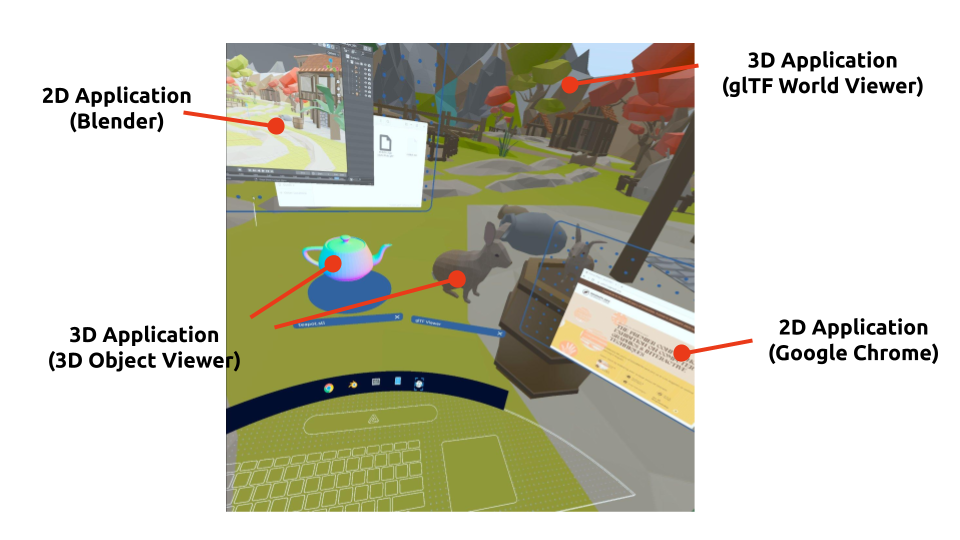
\includegraphics[width=\linewidth]{figure/zwin.png}
  \caption{
    XRコンテンツ制作などの3DワークフローをZwinが支援する様子.
  }
  \label{fig:zwin}
\end{figure}

\begin{figure}[htbp]
  \centering
  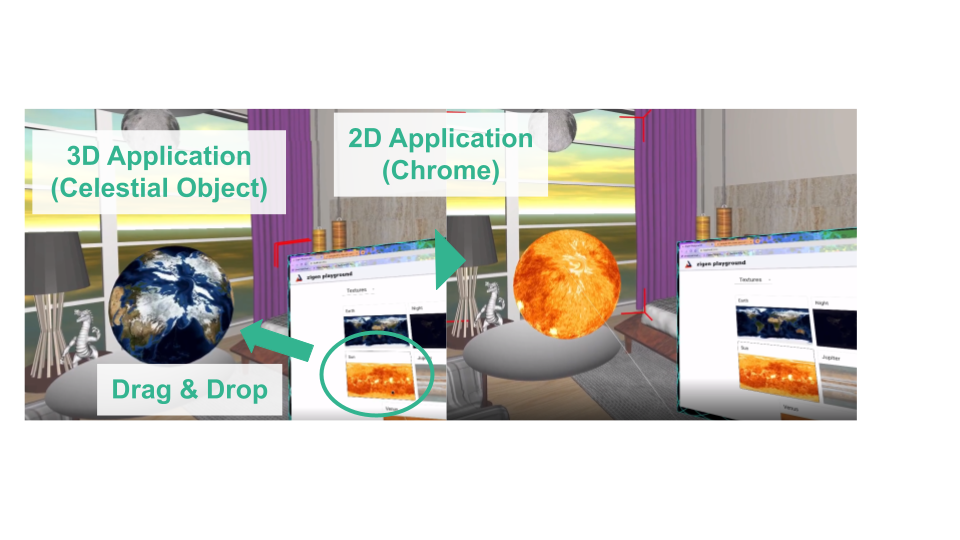
\includegraphics[width=\linewidth]{figure/zwin2.png}
  \caption{
    ブラウザと3Dアプリケーションとの間でのドラッグ \& ドロップの様子.
    天体を表示するアプリケーションにブラウザからテクスチャをドラッグ \& ドロップすることで
    天体の見た目を変えている(図では地球から太陽に変化している).
  }
  \label{fig:zwin2}
\end{figure}

\subsection{実装}

ここでは詳細な仕組みの説明は避けるが,Zwinプロジェクトでは既存の2Dアプリケーション用の
Windowing Systemのプロトコル(ディスプレイサーバとアプリケーションとの間のやりとりのルール)と,
本プロジェクトで新たに定義した3Dアプリケーション用のプロトコルとを実装した
ディスプレイサーバを一から開発している.
また,通常のディスプレイを用いたデスクトップ環境と,VRを用いたデスクトップ環境とを
行き来できるようにしているため,その両方を実装していたり,Meta Questで利用可能にするため,
PCからMeta Questへネットワーク越しにレンダリング情報を送るためのリモートレンダリングシステムを
gRPC上に作成するなどしている.

\section{プロジェクト紹介映像 (Long ver. 8分11秒)}
こちらにはより詳細なコンセプトや使い方が詳しく解説されているので,ご覧いただきたい.

\url{https://youtu.be/uZEDEfEZB1w}

\section{私の役割}

私はプロジェクト全体のリードと開発部分のリードをおこなっている.

開発部分のリードとしては,主に基幹部分の開発と他のエンジニアとのタスクの分離・分配,
コードレビューを通じたOSSとしての文化形成などをおこなっている.

プロジェクト全体のリードとしてはレンダリングやXR,Windowing Systemの仕組みを低レベルから
理解したうえで,デザインやUXを考えているメンバーと話して,XR Windowing Systemとしてあるべき
パラダイムを慎重に検討し,プロトコルを策定したりしている.

\section{Further Information}

\begin{itemize}
  % \item \textbf{プロジェクト紹介映像 (Long ver. 8分11秒)} \\
  %       \url{https://youtu.be/uZEDEfEZB1w} \\
  %       こちらにはより詳細なコンセプトや使い方が詳しく解説されているので,是非ご覧ください.
  \item \textbf{プロジェクトホームページ} \\
        \url{https://www.zwin.dev/}
  \item \textbf{Getting Started} \\
        \url{https://www.zwin.dev/getting_started/system_requirements}
  \item \textbf{Road Map} \\
        \url{https://www.zwin.dev/roadmap}
  \item \textbf{Twitter} \\
        \url{https://twitter.com/zwin_project} \\
        固定ツイートがベータ版のリリース時のツイートになります.
  \item \textbf{Discord} \\
        \url{https://t.co/Vl1fqZyr5i}
  \item \textbf{GitHub} \\
        \url{https://github.com/zwin-project}
\end{itemize}

\end{document}
